\documentclass{article}
\usepackage[margin=0.2cm,paperwidth=24cm,paperheight=14cm]{geometry}
\usepackage{tikz,xcolor}
\usetikzlibrary{decorations.pathreplacing}
\pagestyle{empty}
\begin{document}
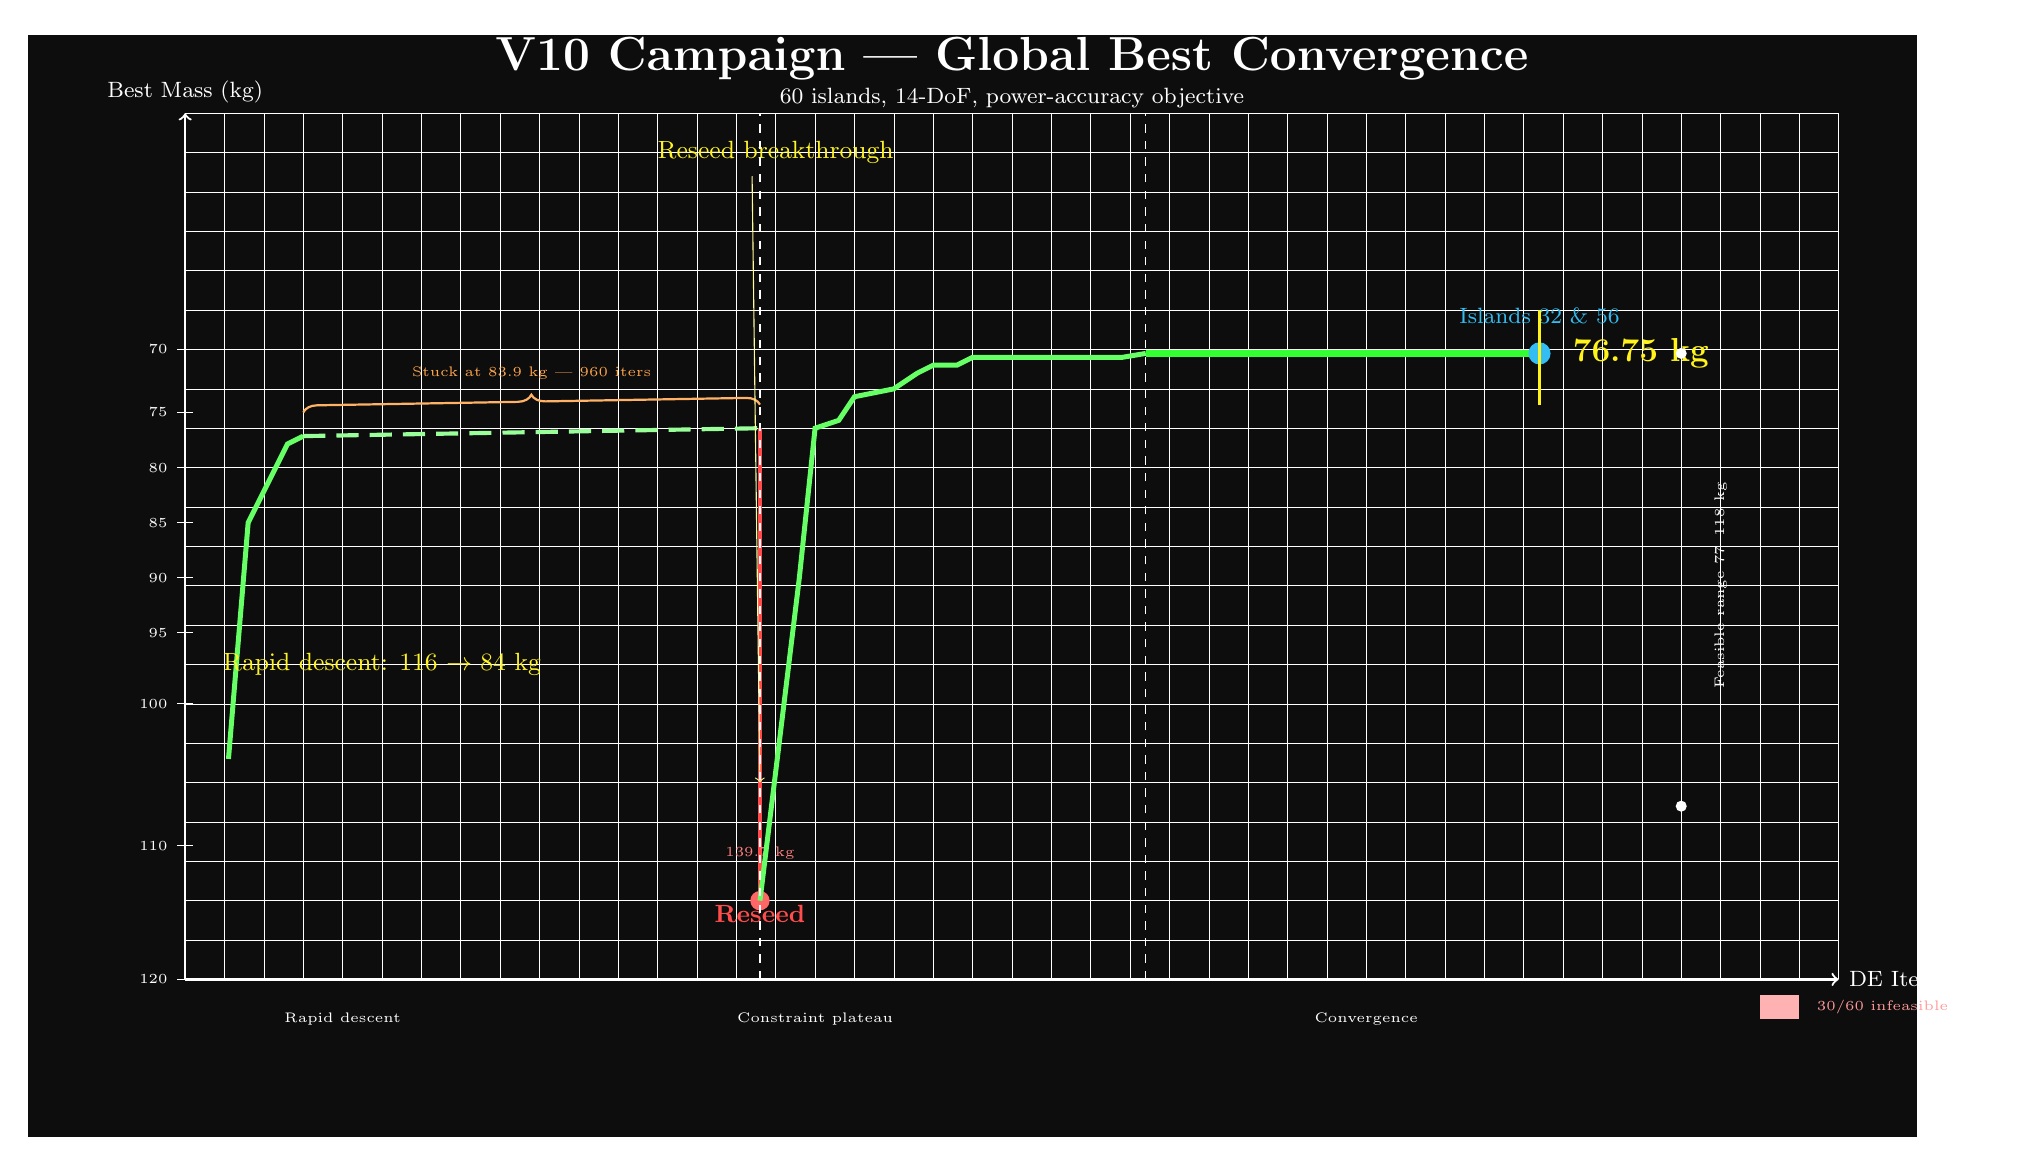
\begin{tikzpicture}[scale=1.0]

\fill[black!95] (0,0) rectangle (24,14);
\draw[white!10, very thin] (2,2) grid[step=0.5] (23,13);
\draw[white!50, line width=0.8pt, ->] (2,2) -- (23,2) node[right, white] {\footnotesize DE Iterations};
\draw[white!50, line width=0.8pt, ->] (2,2) -- (2,13) node[above, white] {\footnotesize Best Mass (kg)};

\foreach \y/\label in {2/120, 3.7/110, 5.5/100, 6.4/95, 7.1/90, 7.8/85, 8.5/80, 9.2/75, 10/70} {
    \draw[white!25, thin] (1.9,\y) -- (2.1,\y);
    \node[white!50, left, font=\tiny] at (1.9,\y) {\label};
}

% Phase labels
\node[white!40, font=\tiny] at (4, 1.5) {Rapid descent};
\node[white!40, font=\tiny] at (10, 1.5) {Constraint plateau};
\node[white!40, font=\tiny] at (17, 1.5) {Convergence};

% ── CURVES ──────────────────────────────────────────────────────────
% Data: (x,y) computed from (iter, mass) → (1.5+iter*15/3000, 1.5+(140-mass)*7.5/70)
% Scaled to new 2..22 range: x*20/16.5

\def\sx{1.212} % scale x from old coords to new range
\def\syy{1.2}  % slight y stretch

% Rapid descent
\draw[green!60!white, line width=1.8pt]
    (2.55,4.8) -- (2.8,7.8) -- (3.0,8.2) -- (3.3,8.8) -- (3.5,8.9);

% Plateau
\draw[green!40!white, line width=1.5pt, dashed, dash pattern=on 8pt off 4pt]
    (3.5,8.9) -- (9.3,9.0);

\draw[orange!60, line width=0.8pt, decorate, decoration={brace, amplitude=5pt}]
    (3.5,9.2) -- (9.3,9.3);
\node[orange!70, font=\tiny, above] at (6.4,9.5) {Stuck at 83.9 kg --- 960 iters};

% Reseed spike
\draw[red!70, line width=1.5pt] (9.3,9.0) -- (9.3,3.0);
\fill[red!60] (9.3,3.0) circle (3.5pt);
\node[red!70, font=\small, above] at (9.3,2.6) {\textbf{Reseed}};
\node[red!50, font=\tiny] at (9.3,3.6) {139.7 kg};

% Post-reseed descent
\draw[green!60!white, line width=1.8pt]
    (9.3,3.0) -- (9.8,7.1) -- (10.0,9.0) -- (10.3,9.1) -- (10.5,9.4)
    -- (11.0,9.5) -- (11.3,9.7) -- (11.5,9.8) -- (11.8,9.8) -- (12.0,9.9)
    -- (12.2,9.9) -- (12.7,9.9) -- (13.3,9.9) -- (13.9,9.9) -- (14.2,9.95);

% Converged flatline
\draw[green!80!white, line width=2.5pt]
    (14.2,9.95) -- (19.2,9.95);

% Confirmation markers
\fill[cyan!80] (19.2,9.95) circle (4pt);
\node[cyan!80, font=\footnotesize, above] at (19.2,10.2) {Islands 32 \& 56};

% Annotations
\node[yellow!85, font=\small] at (4.5,6.0) {Rapid descent: 116 $\rightarrow$ 84 kg};
\node[yellow!85, font=\small, align=center] at (9.5,12.5) {Reseed breakthrough};
\draw[yellow!40, ->, line width=0.4pt] (9.2,12.2) -- (9.3,4.5);

\draw[yellow!90, line width=1.2pt] (19.2,9.3) -- (19.2,10.5);
\node[yellow!90, font=\large\bfseries, right] at (19.5,9.95) {76.75 kg};

% Phase dividers
\draw[white!10, line width=0.5pt, dashed] (9.3, 2) -- (9.3, 13);
\draw[white!10, line width=0.5pt, dashed] (14.2, 2) -- (14.2, 13);

% Other islands
\draw[white!25, line width=0.4pt] (21, 4.2) -- (21, 9.95);
\fill[white!20] (21, 4.2) circle (2pt);
\fill[white!20] (21, 9.95) circle (2pt);
\node[white!40, font=\tiny, rotate=90] at (21.5, 7.0) {Feasible range 77--118 kg};

\fill[red!30] (22, 1.5) rectangle (22.5, 1.8);
\node[red!40, font=\tiny, right] at (22.6, 1.65) {30/60 infeasible};

\node[white, font=\LARGE\bfseries] at (12.5, 13.7) {V10 Campaign --- Global Best Convergence};
\node[white!50, font=\footnotesize] at (12.5, 13.2) {60 islands, 14-DoF, power-accuracy objective};

\end{tikzpicture}
\end{document}
